%\documentclass[margin=0pt]{standalone}
%\usepackage{tikz}
\usetikzlibrary{arrows.meta}

\begin{document}

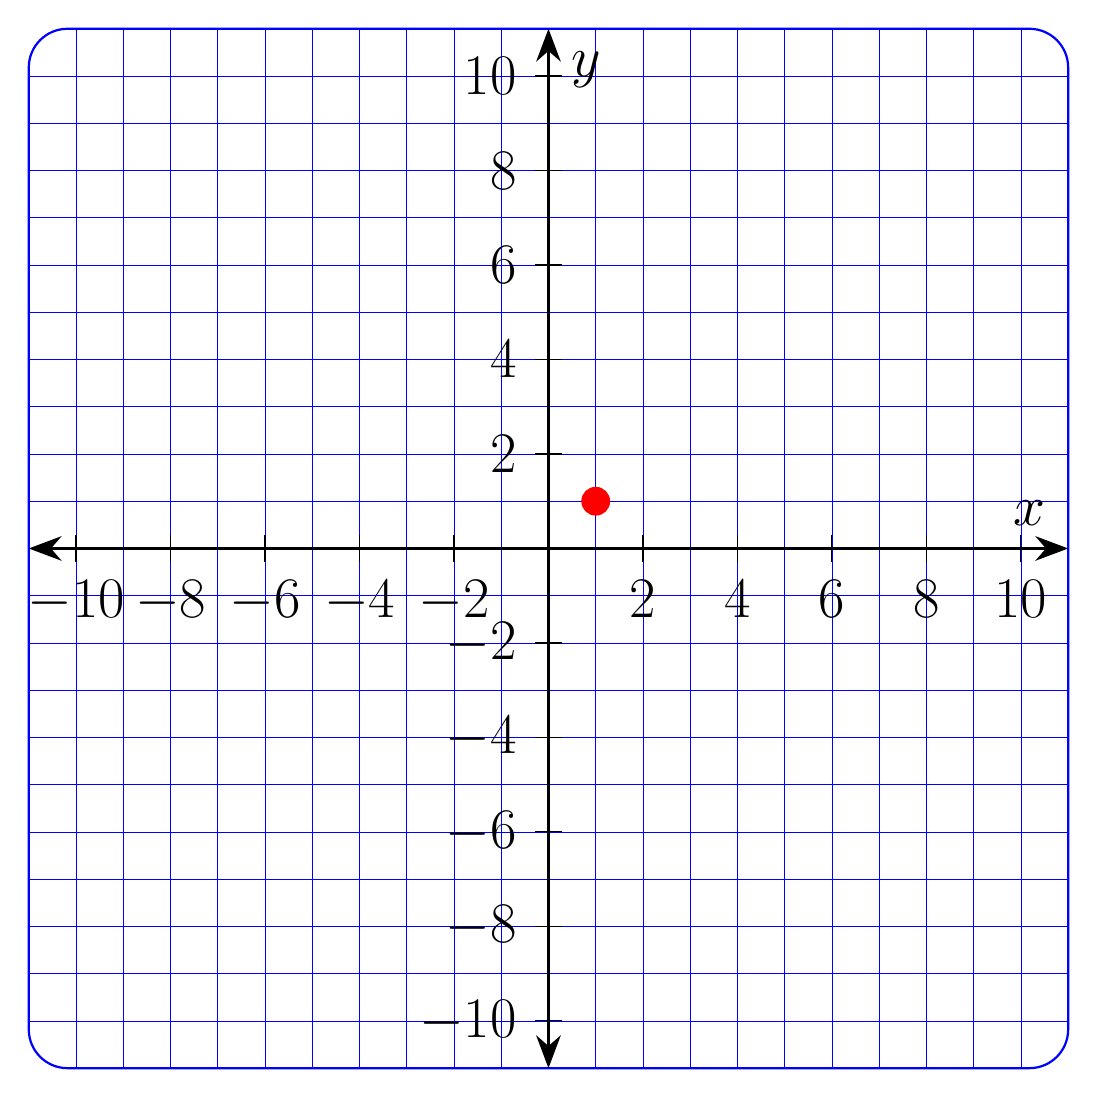
\begin{tikzpicture}[x=0.6cm,y=0.6cm]
\tikzset{>={Stealth[scale=1.8]}}
\filldraw[draw=blue,fill=white,rounded corners=14pt,thick,use as bounding box] (-11,-11) rectangle (11,11);
\foreach \x in {-10,...,10} {
	\draw [line width=0.2pt, color=blue] (\x,-11) -- (\x,11);
}
\foreach \y in {-10,...,10} {
	\draw [line width=0.2pt, color=blue] (-11,\y) -- (11,\y);
}
\huge
\draw[<->,thick] (-11,0) -- (11,0) node[above left,outer sep=2pt]{$x$};
\draw[<->,thick] (0,-11) -- (0,11) node[below right,outer sep=2pt]{$y$};
\foreach \x in {-10,-8,...,-2,2,4,...,10} \draw[thin] (\x,5pt) -- (\x,-5pt) node[below]{$\x$};
\foreach \y in {-10,-8,...,-2,2,4,...,10} \draw[thin] (5pt,\y) -- (-5pt,\y) node[left]{$\y$};
\filldraw[red] (1,1) circle[radius=5pt];
\end{tikzpicture}

\end{document}
